
%(BEGIN_QUESTION)
% Copyright 2006, Tony R. Kuphaldt, released under the Creative Commons Attribution License (v 1.0)
% This means you may do almost anything with this work of mine, so long as you give me proper credit

A pump pushes liquid kerosene ($\rho$ = 1.59 slugs/ft$^{3}$) through a piping system.  Calculate the pressure measured at the gauge, assuming a pump discharge pressure of 45.1 PSI and a discharge flow of 250 GPM:

$$\includegraphics[width=15.5cm]{i00049x01.eps}$$

\vfil 

\underbar{file i00049}
\eject
%(END_QUESTION)





%(BEGIN_ANSWER)

This is a graded question -- no answers or hints given!

%(END_ANSWER)





%(BEGIN_NOTES)

This is nothing more than an exercise in applying Bernoulli's equation, with all the necessary unit conversions.  {\it Let the fun begin:}

\vskip 10pt

$P_1$ = 45.1 PSI = 6494.4 PSF

\vskip 10pt

$Q$ = 250 GPM = 57750 in$^{3}$/min = 33.42 ft$^{3}$/min = 0.55700 ft$^{3}$/s

\vskip 10pt

$A_1$ = Flowing area of 10" pipe = 0.54542 ft$^{2}$

\vskip 10pt

$A_2$ = Flowing area of 4" pipe = 0.087266 ft$^{2}$

\vskip 10pt

$v_1$ = Kerosene velocity at 10" pipe = $Q \over A_1$ = 1.02124 ft/s

\vskip 10pt

$v_2$ = Kerosene velocity at 4" pipe = $Q \over A_2$ = 6.38278 ft/s

% No blank lines allowed between lines of an \halign structure!
% I use comments (%) instead, so Tex doesn't choke.

$$\vbox{\offinterlineskip
\halign{\strut
\vrule \quad\hfil # \ \hfil & 
\vrule \quad\hfil # \ \hfil & 
\vrule \quad\hfil # \ \hfil \vrule \cr
\noalign{\hrule}
%
% First row
{\bf Head} & {\bf Calculation} (at 10 inch pipe) & {\bf Value} \cr
%
\noalign{\hrule}
%
% Another row
$z_1 \rho g$ & (0 ft) (1.59 slugs/ft$^{3}$) (32.2 ft/s$^{2}$) & 0 lb/ft$^{2}$ \cr
%
\noalign{\hrule}
%
% Another row
$v_1^2 \rho / 2$ & (1.02124 ft/s)$^{2}$ (1.59 slugs/ft$^{3}$) / 2 & 0.829137 lb/ft$^{2}$ \cr
%
\noalign{\hrule}
%
% Another row
$P_1$ & (45.1 lb/in$^{2}$) (144 in$^{2}$/1 ft$^{2}$) & 6494.4 lb/ft$^{2}$ \cr
%
\noalign{\hrule}
%
% Another row
{\bf Total} &  0 lb/ft$^{2}$ + 0.829137 lb/ft$^{2}$ + 6494.4 lb/ft$^{2}$ & {\bf 6495.229 lb/ft$^{2}$} \cr
%
\noalign{\hrule}
} % End of \halign 
}$$ % End of \vbox

% No blank lines allowed between lines of an \halign structure!
% I use comments (%) instead, so Tex doesn't choke.

$$\vbox{\offinterlineskip
\halign{\strut
\vrule \quad\hfil # \ \hfil & 
\vrule \quad\hfil # \ \hfil & 
\vrule \quad\hfil # \ \hfil \vrule \cr
\noalign{\hrule}
%
% First row
{\bf Head} & {\bf Calculation} (at 4 inch pipe) & {\bf Value} \cr
%
\noalign{\hrule}
%
% Another row
$z_2 \rho g$ & (-5 ft) (1.59 slugs/ft$^{3}$) (32.2 ft/s$^{2}$) & -255.99 lb/ft$^{2}$ \cr
%
\noalign{\hrule}
%
% Another row
$v_2^2 \rho / 2$ & (6.38278 ft/s)$^{2}$ (1.59 slugs/ft$^{3}$) / 2 & 32.3882 lb/ft$^{2}$ \cr
%
\noalign{\hrule}
%
% Another row
$P_2$ &  & (unknown) \cr
%
\noalign{\hrule}
%
% Another row
{\bf Total} &  -255.99 lb/ft$^{2}$ + 32.3882 lb/ft$^{2}$ $+ P_2$ & {\bf -223.6018 lb/ft$^{2}$} $+ P_2$ \cr
%
\noalign{\hrule}
} % End of \halign 
}$$ % End of \vbox

$6495.229 = -223.6018 + P_2$

\vskip 10pt

$P_2$ = Pressure at 4" pipe = 6718.8310 PSF = {\bf 46.65855 PSI}

\vskip 10pt

{\it Now, wasn't that fun??!!}

%INDEX% Physics, dynamic fluids: Bernoulli's equation

%(END_NOTES)


